\documentclass[]{nsm-thesis}
% options:
% [germanthesis] - Thesis is written in German
% [plainunnumbered] - Don't print numbers on plain pages
% [earlydraft] - Settings for quick draft printouts
% [watermark] - Print current time/date at bottom of each page
% [phdthesis] - switch to PhD thesis style
% [twoside] - double sided
% [cutmargins] - text body fills complete page

% Author name. Separate multiple authors with commas.

\usepackage{acro}
\usetikzlibrary{quotes,angles}


\author{Karl Christian Lautenschläger}
\birthday{29. Juni 1998}
\birthplace{Magdeburg}

% Title of your thesis.
\title{Suitability of Modern Wi-Fi for Wireless-Infield-Communication of Agricultural	Machines}

% Choose one of the following lines, changing the word "Computer Science" to match your degree program.
\thesistype{Diploma Thesis in Information Systems Engineering}\thesiscite{Diploma Thesis~(Diplomarbeit)}

\advisors{Christoph Sommer}
% List of advisors (without academic titles), separated by commas.

% List of referees (without academic titles), separated by commas.
\referees{Christoph Sommer, Burkhard Hensel}

\DeclareAcronym{FH}{
	short=FH,
	long=Forage Harvester,
}
\DeclareAcronym{TM}{
	short=TM,
	long=Transport Machine,
}

\DeclareAcronym{FEC}{
	short=FEC,
	long=Forward Error Correction,
}
\DeclareAcronym{WPA}{
	short=WPA,
	long=Wi-Fi Protected Access,
}

\DeclareAcronym{DCF}{
	short=DCF,
	long=Distribution Coordination Function,
}
\DeclareAcronym{DIFS}{
	short=DIFS,
	long=Distributed Coordination Function Interframe Space,
}
\DeclareAcronym{SSID}{
	short=SSID,
	long=Service Set Identifier,
}
\DeclareAcronym{SIFS}{
	short=SIFS,
	long=Short Interframe Space,
}
\DeclareAcronym{ACK}{
	short=ACK,
	long=Acknowledgement,
}
\DeclareAcronym{NAV}{
	short=NAV,
	long=Network Allocation Vector,
}
\DeclareAcronym{PCF}{
	short=PCF,
	long=Point Coordination Function,
}
\DeclareAcronym{CSMACA}{
	short=CSMA/CA,
	long=Carrier Sense Multiple
	Access/Collision Avoidance,
}

\DeclareAcronym{IBSS}{
	short=IBSS,
	long=Independent Basic Service Set,
}
\DeclareAcronym{AP}{
	short=AP,
	long=Access Point,
}
\DeclareAcronym{WIC}{
	short=WIC,
	long=Wireless-Infield Communication,
}
\DeclareAcronym{M2M}{
	short=M2M,
	long=Machine-To-Machine,
}

\DeclareAcronym{MIMO}{
	short=MIMO,
	long=Multiple Input Multiple Output,
}
\DeclareAcronym{MCS}{
	short=MCS,
	long=Modulation
	and Coding Scheme,
}
\DeclareAcronym{GI}{
	short=GI,
	long=Guard Interval,
}
\DeclareAcronym{MANET}{
	short=MANET,
	long=Mobile Ad Hoc Network
	and Coding Scheme,
}  

\DeclareAcronym{ASC}{
	short=ASC,
	long=Automatic Section Control,
}
\DeclareAcronym{m-ASC}{
	short=m-ASC,
	long=Meshed Automatic Section Control,
}
\DeclareAcronym{AEF}{
	short=AEF,
	long=Agricultural Industry Electronics Foundation,
}
\DeclareAcronym{FMIS}{
	short=FMIS,
	long=Farm Management Information System,
}
\DeclareAcronym{hTMM}{
	short=hTMM,
	long=Hybrid Threat Modeling Method,
}
\DeclareAcronym{STRIDE}{
	short=STRIDE,
	long= Spoofing\, Tampering\, Repudiation\, Information disclosure\, Denial of services\, and Escalation
	of privileges,
}
\DeclareAcronym{PASTA}{
	short=PASTA,
	long= Process for Attack Simulation and Threat Analysis,
}

\DeclareAcronym{ac}{
	short=802.11ac,
	long= IEEE 802.11ac,
}

\DeclareAcronym{ax}{
	short=802.11ax,
	long= IEEE 802.11ax,
}

\DeclareAcronym{OFDMA}{
	short=OFDMA,
	long= Orthogonal Frequency-Division Multiple Access,
}
\DeclareAcronym{OFDM}{
	short=OFDM,
	long= Orthogonal Frequency-Division Multiplexing,
}
\DeclareAcronym{RU}{
	short=RU,
	long= Resource Unit,
}
\DeclareAcronym{SINR}{
	short=SINR,
	long= Signal-to-Interference-plus-Noise Ratio,
}
\DeclareAcronym{QAM}{
	short=QAM,
	long=Quadrature Amplitude Modulation,
}
\DeclareAcronym{PSK}{
	short=PSK,
	long=Phase Shift Keying,
}
\DeclareAcronym{RSS}{
	short=RSS,
	long=Received Signal Strength,
}
\DeclareAcronym{PDR}{
	short=PDR,
	long=Packet Delivery Ratio,
}
\DeclareAcronym{LOS}{
	short=LOS,
	long=Line-of-sight,
}
\DeclareAcronym{ESS}{
	short=ESS,
	long=Extended Service Set,
}
\DeclareAcronym{BSS}{
	short=BSS,
	long=Basic Service Set,
}


% Define abbreviations used in the thesis here.
\acrodef{WSN}{Wireless Sensor Network}

\acrodef{ROI}{Region of Interest}{short-indefinite={an}, long-plural-form={Regions of Interest}}
\acrodef{ADAC}{German Automobile Association}{foreign={Allgemeiner Deutscher Automobilclub}}
\acrodef{CANhashing}[CAN]{Content Addressable Network}{extra={when referring to the distributed hash table}}
\acrodef{CANproto}[CAN]{Controller Area Network}{extra={when referring to the bus protocol}}

\begin{document}

\pagenumbering{roman}

\maketitle

\cleardoublepage

\TODO{This template is for use with \texttt{pdflatex} and \texttt{biber}. It has been tested with TeX~Live 2020 (as of 25 Oct 2020).}

\chapter*{Abstract}
\addcontentsline{toc}{chapter}{Abstract}
\begin{otherlanguage*}{american}

about 1/2 page:
\begin{enumerate}
    \item Motivation (Why do we care?)
    \item Problem statement (What problem are we trying to solve?)
    \item Approach (How did we go about it)
    \item Results (What's the answer?)
    \item Conclusion (What are the implications of the answer?)
\end{enumerate}

The abstract is a miniature version of the thesis.
It should be treated as an entirely separate document.
Do not assume that a reader who has access to an abstract will also have access to the thesis.
Do not assume that a reader who reads the thesis has read the abstract.

\end{otherlanguage*}


\chapter*{Kurzfassung}
\addcontentsline{toc}{chapter}{Kurzfassung}
\begin{otherlanguage*}{ngerman}

Gleicher Text (sinngemäß, nicht wörtlich) in Deutsch

\end{otherlanguage*}
\acresetall

\cleardoublepage
\tableofcontents
\TODO{The table of contents should fit on one page. When in doubt, adjust the \texttt{tocdepth} counter.}

\cleardoublepage
\pagenumbering{arabic}


\chapter{Introduction}
%\chapter{Einleitung}
\label{sec:introduction}

\begin{itemize}
\item general motivation for your work, context and goals.
\item context: make sure to link where your work fits in
\item problem: gap in knowledge, too expensive, too slow, a deficiency, superseded technology
\item strategy: the way you will address the problem
\item recommended length: 1-2 pages.
\end{itemize}




\chapter{Fundamentals}
\label{sec:fundamentals}



\begin{itemize}
\item describe methods and techniques that build the basis of your work
\item include what's needed to understand your work (e.g., techniques, protocols, models, hardware, software, ...)
\item exclude what's not (e.g., anything you yourself did, anything your reader can be expected to know, ...)
\item review related work(!)
\item recommended length: approximately one third of the thesis.
\end{itemize}

\TODO{
	-1/3 ist kurz, weil der Bezug und die Relation zur Landwirtschaft groß ist... Aber wen interessiert das? 
-1/3  related Work erwähnt man dann Unterstützung von Professor Klingler wie und wo? erwähnt man sich selber ?  
`}
\section{\acl{WIC}}
Given that there are many different agricultural technology companies worldwide and  mix of their machines is often used together in an agricultural company, a demand for interoperability between agricultural machines of different brands emerged. In 2008, the \ac{AEF} was founded to develop and standardize this interoperability w\footnote{https://www.aef-online.org/about-us/about-the-aef.html Accessed: 24.07.2022}.

The AEF has defined a binary unit system, the ISO 11783 standard, for agricultural machinery communication, mainly tractors and implements \cite{iglesias_enabling_2014}. According to \textcite{schlingmann_aef_2019}, the ISO 11783 standard is known as the ISOBUS system.

The authors mention that the AEF is currently working on other issues. Among them is also the \ac{WIC}. In the associated project group \ac{WIC}, solutions for \ac{M2M} communication between cooperating, agricultural machines are to be developed and standardized.

For this purpose, the authors name the following use cases:
\todo[color=blue]{Den Teil haben mehrere Leute Korrektur gelesen. Den musst du nicht überfliegen, da man ihn kaum für das Verständnis braucht.}
Since 2014, the \ac{WIC} project group has been working on the development of a for \ac{WIC} standard, which covers a standard for machine-to-machine communication, encryption, and security \footnote{https://www.aef-online.org/about-us/teams.html}.
\textcite{schlingmann_aef_2019} summarize the goals of the \ac{WIC} project team as follows:
\begin{itemize}
	\item Define use cases for \ac{WIC} in agriculture
	\item Evaluate the suitability of communication technologies
	\item Find suitable communication protocols
	\item Standardize the \ac{WIC} common software library
	\item Develop functional and security requirements and concepts
	\item Test first prototypes in regards of cross-brand comformance
	\item Write a application guideline
\end{itemize}
First steps have already been taken in this direction. The use cases and key scenarios are defined and explained by the authors as follows:
\begin{itemize}
	\item \textbf{Real-Time Machine-to-Machine Control} is the exchange of control data under real-time conditions with defined latency policies. This use case enables leader-follower scenarios where agricultural machines follow a leading agricultural machine at a lateral and longitudinal distance. Throughout this thesis, I will refer to Real-Time Machine-to-Machine Control as Agricultural Platooning Service.
	%\TODO{Fendt-Paper? Auch erwähnen eigentlich ja später, Beispiel aus AEF Paper?}
	\item \textbf{Streaming Services} are communications that stream video from remote cameras and monitors at a high data rate and low latency. The authors estimate the distance between the communication participants to be less than \SI{100}{\metre}. As a result, this data is available on another agricultural vehicle and can be analyzed and processed there.
	I will refer to Streaming Services as Agricultural Streaming Services in this thesis. %\TODO{Camera harvest streaming}
	\item \textbf{Process Data Exchange} describes the exchange of process data. One example is the exchange of already sprayed field areas to prevent multiple spraying of fertilizers and pesticides on the same field area by different machines. According to the authors, this \ac{WIC} use case requires long-range technologies because agricultural fields worldwide can be vast.
	%\TODO{ISO 11783-10 extended FMIS Data Interface}
	\item \textbf{Fleet Management \& Logistics} is the potential retrieval of data from the ongoing agricultural process. This information can influence economic or agronomic decisions of agricultural enterprises or service companies and is therefore required in a \ac{FMIS}.
	Since not all agricultural machines may be connected to the \ac{FMIS}, the \ac{WIC} project group is looking at how to use \ac{M2M} communications to bridge the missing communications infrastructure until the data reaches a machine that can connect to the \ac{FMIS}.
	\item \textbf{Road Safety} describes a use case which is already a project between the European Telecommunication Standard Institute and the \ac{AEF}. Since agricultural vehicles are repeatedly underestimated in their size and speed by other road users when they suddenly turn off the field onto the road, the other road users need to be warned in this situation. In this way, smart technologies in cars and motorcycles can brake these vehicles in advance and prevent possible accidents.
\end{itemize}

\todo[color=blue]{Wichtig:}
Considering that I investigate the Suitability of modern Wi-Fi for Wireless-Infield-Communication and modern Wi-Fi like IEEE 802.11ax is no long range technologies,
I will focus on investigating the suitability of IEEE 802.11ax for the \ac{WIC} use case Real-Time Machine-to-Machine Control.
Throughout this thesis, I will refer to real-time machine-to-machine control as Agricultural Platooning.
An example how farmers can benefit from Streaming Services or Agricultural Platooning Services is the corn harvesting and loading process.


Considering that I investigate the Suitability of modern Wifi for Wireless-Infield-Communication and Wi-Fi 6 and Wi-Fi 5 are no long range technologies, I will focus on investigating the suitability of these two Wi-Fi standards for the \ac{WIC} use cases Real-Time Machine-to-Machine Control and Streaming Services. Throughout this thesis, I will refer to real-time machine-to-machine control as Agricultural Platooning.
\section{Related Work}
AEF Vorgehen

Lösungen
Technologien

Außer AEF Platooning:

	OMNiDRIVE Raven Industries Technology? Starfire In einem Manual?
	Machine Sync Starfire 6000 - SF1 Gen4 4240 Display Autotrac 300 
	CartACE Nothing named? 
	
	AutoSync Trimble m-ASC

Außer AEF Video Streaming:

	OcuSync
	Lightbridge DJI Mavic
	Herelink

\todo{What is it? 2.4 GHz? But is it Wifi? }

In order to implement these described \ac{WIC} use cases, the \ac{WIC} project group has been searching for a technology that can realize the required data rates, latencies and high transmission range. The plans for doing so are written down by members of the \ac{WIC} project group in \cite{schlingmann_challenges_2017}.

The authors consider the fundamental use of cellular networks as very problematic because, according to \cite{noauthor_ict_2016}, only \SI{30}{\percent} of the land surface has network coverage. For this reason, there is a major concern that the required data cannot be exchanged because there is no network connectivity in many fields. Nevertheless, the authors want to leave the future \ac{WIC} system open to cellular standards.

The current focus of the authors is on IEEE 802.11 technologies, which must first be evaluated for use in the agricultural environment.

In collaboration with \textcite{klingler_agriculture_2018}, the authors investigated IEEE 802.11p technology for \ac{WIC} in agricultural scenarios. Experiments revealed that data could be exchanged over a maximum range of \SI{1700}{\metre}. But during the measurement in an agricultural work scenario from the corn harvest, there were collapses in the Received Signal Strength due to shadowing effects of the machines. The high range, data rate, and possible latencies make IEEE 802.11p a good technology for \ac{WIC} according to \textcite{schlingmann_challenges_2017}.

As of July 2, 2021, the frequency spectrum of IEEE 802.11p in the United States of America, ranging from \SIrange{5,850}{5,925}{\giga\hertz}, has been split. The upper \SI{30}{\mega\hertz} are reserved for Intelligent transportation systems now. The lower \SI{45}{\mega\hertz} have been released for unlicensed operations \cite{noauthor_use_2021}.

Since the use of IEEE 802.11p has now been newly regulated by the FCC, the \ac{WIC} project group is looking for an alternative technology that enables \ac{WIC}.
\section{Wireless Lans according to IEEE 802.11}
\todo{Paper Christoph Sommer, Doktorarbeit, Diplomarbeit, Mario Franke, Tobias Hardes}
According to \textcite{kauffels_wireless_2002} the first version of the Standard IEEE 802.11 was published in 1999 to enable a wireless alternative to Ethernet - or Token-Ring - networks.
\textcite{sauter_wireless_2022} considers IEEE 802.11 also to be an implementation of Ethernet with the help of wirless radio technologies. The author lists the extensions to the original standard, which range from 802.11b, 802.11g, 802.11a, 802.11n, 802.11ac to the latest enhancement 802.11ax. The different IEEE 802.11 standards can operate in the  \SI{2.4}{\giga\hertz} - , \SI{5}{\giga\hertz} and \SI{6}{\giga\hertz} - frequency band. 


\textcite{kauffels_wireless_2002} defines the following three basic architectures for IEEE 802.11.

If two or more stations communicate directly without an AP, they form an ad hoc network. According to the author, this can be set up quickly and easily and is also called \ac{IBSS}.

The Infrastructure \ac{BSS} mode allows all stations within the range of defined range around the \ac{AP} to communicate via a central \ac{AP}. Within the area of the \ac{BSS}, all stations can move freely and communicate with one another.

Since an \ac{AP} has limited range and can only cover a certain area, the \ac{ESS} was introduced. It contains a distribution system, which links several \ac{BSS} with each other.

Thereby, the BSS coverage areas can physically overlap so that continuous connection of stations within the ESS can be provided. For a better performance the \ac{BSS} can be placed physically on top of each other. One can also have physically separate \ac{BSS}s so that these \ac{BSS}s can be linked together over long distances. According to the author, the standard does not specify a distance limit for such connections. 

He also mentions, that the standard defines the following three mobility types for station in an \ac{ESS}, where a station can do no-transition and thereby stay within a \ac{BSS}, \ac{BSS}-transitioning and move from one \ac{BSS} to another \ac{BSS} within the same \ac{ESS} and \ac{ESS}-transition, where the Station moves from a \ac{ESS} to another one but no stable connection can be guaranteed.

\textcite{sauter_wireless_2022} adds, that usually Ethernet is used to link \ac{AP}s in within an \ac{ESS}. But according to the author this can be replaced by a wireless connection, which is called wireless bridge.
\TODO{Sauter 2022 Ad-Hoc Infos}
The further development of IEEE 802.11 is accompanied by a constant change of the physical layer. \textcite{sauter_wireless_2022} mentions, that all new enhancements of the physical layer of IEEE 802.11 are backward compatible to previous definitions of the it.

According to the Author, IEEE 802.11 initially used DSSS and FHSS as modulation methods.
Since IEEE 802.11g the modulation method \ac{OFDM} can be used in the \SI{2.4}{\giga\hertz} frequency band. \ac{OFDM} divides the transmission channel in subcarriers with different amplitudes, frequencies and phases. Each subcarrier is orthogonal to another one, as they send the information "Low", where only one other subcarrier is sending the information "High".
For the modulation and demodulation the FFT and IFFT are used respectively.
\textcite{kauffels_wireless_2002} states, that \ac{OFDM} can be used in the \SI{5}{\giga\hertz} frequency band since IEEE 802.11a.

Convolutional encoders are used to increase redundancy. This enables \ac{FEC}, which can distribute a bit sequence over the \ac{OFDM} subcarriers in such a way that an original bit sequence can be decoded at the receiver even in the event of interference. \textcite{kauffels_wireless_2002}


Various \ac{MCS}s can be selected in the physical layer in order to transmit as many bits as possible in the signal. 
These \ac{MCS}s are based on \ac{PSK} or \ac{QAM}. 
\textcite{kauffels_wireless_2002} recommends setting the parameters in an \ac{OFDM} system in such a way that first the coding rate and then the complexity of the \ac{MCS} is reduced in difficult transmission environments.\TODO{Viel aus gleichem Lehrbuch Quellen? / Lieblingsautor / }
An imaginary, theoretical transmission channel is usually specified as a square-wave signal in the frequency domain with the limits of both minimum and maximum amplitude and cut-off frequency. \textcite{kauffels_wireless_2002} defines the roll-off factor as a cosine-shaped flattening of the square signal between 0 and 1. In addition, the author points out that \ac{QAM} can generate high roll-off factors, so that signals interfere significantly more with adjacent channels.
The author recommends increasing the frequency spacing between transmission channels.
\todo{Symbol length, GI, subcarrier spacing reciprocal}
\todo{Wellenausbreitung, Überlagerungseffekte, Reflexsion, Reflexsion nicht bei Metall}
\todo{Knauffel OFDM PHY}





The next layer in the OSI model is the Data Link Layer.
The Data Link Layer consists of Medium Access - and Logic Link Control functionalities.


According to \textcite{kauffels_wireless_2002}, the medium access control functionalities cover network entry - ,network authentication - and media access methods.
The author explains, that every \ac{AP} send beacon frames periodically to synchronise its stations in the \ac{BSS} and that the beacon frame contains the \ac{SSID}, which identifies the \ac{BSS} or \ac{ESS} of the station. \textcite{sauter_wireless_2022} adds that a beacon frame contains a \SI{16}{\bit} - long capability information element. Each bit here signals that the \ac{AP} provides a particular function or has a specific feature. 

\textcite{kauffels_wireless_2002} explains the procedure for network entry of a station. A station can use the passive or the active scanning mode. In passive scanning mode, the station listens for a beacon frame in the various transmission channels. Alternatively, in active scanning mode, a station can also send out a probe frame. This can contain an already known \ac{SSID} to test the presence of the \ac{AP}. To get an \ac{AP} in range, the probe-frame can also contain a broadcast SSID that causes all nearby \ac{AP}s to respond. The response of an \ac{AP} to the probe frame is the probe-response frame, which contains the same information as a beacon frame. With the information from the beacon frame, a station can start the authentication process.
 
For this process, \textcite{kauffels_wireless_2002} names the two methods Open System Authentication and Shared Key Authentication. \textcite{sauter_wireless_2022} explains that Open System Authentication is based on a device making an authentication request to the \ac{AP}. If the \ac{AP} answers with a positive status in the Authentication Frame, the station is included in the \ac{BSS}. The actual encryption and authentication is then performed by the \ac{WPA} functions. The author points out that Shared Key Authentication is no longer used today. 

 the IEEE 802.11 standard describes the two media access methods \ac{DCF} and \ac{PCF}.

\textcite{sauter_wireless_2022} explains that \ac{DCF} is based on the media access method \ac{CSMACA}. In \ac{CSMACA} a device that is willing to transmit senses in the air transmission medium for a transmitting activity. If no other device is transmitting, the device can transmit. In the case of transmit activity, the terminal must wait at least until the transmission and \ac{DIFS} are over.
Since data transmission via the air transmission medium is very vulnerable to errors, the standard IEEE 802.11 requires that each received packet must be confirmed with an \ac{ACK} frame.
The \ac{DIFS} ensures that an \ac{ACK} frame can be sent before another station uses the same channel to send a data frame. 
To avoid multiple devices transmitting at the same time after \ac{DIFS}, each ready-to-transmit device determines a random backoff time. The device with the shortest backoff time transmits next and all other ready-to-transmit devices restart the media access procedure. In case two devices start sending next because they both randomly chose the shortest backoff time, the transmitted signal will interfere and the packets will not be answered with an \ac{ACK} frame.
In case of such a faulty transmission, the backoff time of the ready-to-transmit devices can increase exponentially afterwards.

To share the knowledge of a transmission time and the subsequently interframe space, a packet contains a \ac{NAV} that specifies the time the air transmission medium is used.

In various network architectures the "hidden station"-problem may occur. As you can see in \autoref{fig:hidden_station}, Station A is not able to sense a transmission of station B and vise versa. In case of simultaneous transmission of both stations, interference around the \ac{AP} may occur. 
\begin{figure}%
	\centering
	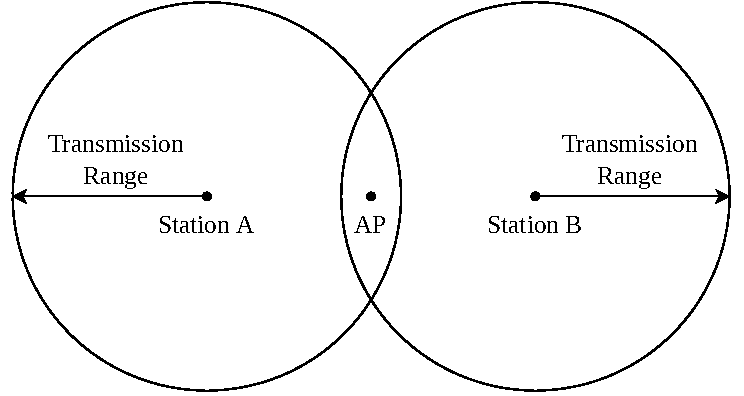
\includegraphics[width=0.75\textwidth]{figures/hidden_station.pdf}
	\caption{Hidden Station Problem}%
	\label{fig:hidden_station}%
\end{figure}
Um das hidden station problem zu umgehen kann eine Station nach \textcite{sauter_wireless_2022} 
Point coordinator 
ohne Wettbewerb mit optionaler Priorisierung

PIFS interval kürzer, 
beacon frame
CF Parameter set-element
\todo{nicht genauer eingehen, weil nicht relevant für die Arbeit? Darf ich das schreiben?}

CSMA /CA
Point Coordination Function

\textcite{sauter_wireless_2022}
DCF oberbegriff für CSMA /CA
 
 
Short Interframe Space SIFS ACK Frame 
 
Hidden Station Problem 
CTS and RTS
 
IEEE 802.11e DCF erweiterung für Video Streaming

CSMA CA Backoff zeit
Network allocation Vector NAV Zeitspanne Datensendungsdauer

MAC Header

Netzeintritt:
passives und Aktives Scanning
Service Set Identifier
Timing Synchronisationsfunktion TSF Timer-Wert

\textcite{sauter_wireless_2022}
every package management or usage data send ackknowledgement

Hidden Station Szenario
Reservieren
RTS CTS
meist nicht konfiguriert / ausgeschalten, bei großen Paketen sinnvoll



Authentifizierung
- Open System -Authentification
- Shared key Authentification
(nach neu nicht mehr verwendet


\subsection{IEEE 802.11ac - Wi-Fi 5}
The 5th generation WLAN is \ac{ac} and operates in the \SI{5}{\giga\hertz}  frequency range \cite{dhawankar_throughput_2018}.

According to \textcite{perahia_gigabit_2011}, \ac{ac} is a further evolution of IEEE 802.11n, where \ac{ac} adds to the known bandwidth of \text{IEEE 802.11n} of \SI{40}{\mega\hertz} the bandwidths \SI{80}{\mega\hertz},\SI{160}{\mega\hertz} and the interrupted bandwidth of \SI{80}{\mega\hertz} + \SI{80}{\mega\hertz}.

nach \textcite{sauter_wireless_2022} ist die Aufspaltung in zwei 80 Mhz Kanäle sehr nützlich, wenn das frequenzband reservierte Regionen enthält. Dadurch kann ein 160 Mhz breiter Kanal um  eine reservierte region des frequenzbandes gebaut werden.

The modulation technique used is \ac{OFDM}.
Additionally, a new \ac{MIMO} Downlink functionality for multiple users, called DL MU-MIMO, with up to 8 partial streams is introduced according to the authors. Together with the new \ac{MCS} from 64 \ac{QAM} to 256 \ac{QAM}, these three enhancements ensure that a higher data rate can be achieved. The maximum data rate is \SI{6.9}{\giga\hertz} according to the authors.

As declared by \textcite{abdelrahman_comparison_2015}, the 5th generation of WLAN has made it possible to expect better performance as in addition to a longer communication range compared to the previous IEEE 802.11 standards This statement could be proven at least for indoor range.  \textcite{dhawankar_throughput_2018} were able to demonstrate that \ac{ac} with a range of over \SI{60}{\metre} enables a longer indoor communication range than previous IEEE 802.11 standards.


new Physical Layer Very High Throughput (VHT) Physical Layer

80 Mhz

Beamforming 

\subsection{IEEE 802.11ax - Wi-Fi 6}

The 6th generation of WLAN is \ac{ax}. \textcite{khorov_tutorial_2019} reveals what has changed from \ac{ac} to \ac{ax}. For this, the authors make the following statements.

\ac{ax} uses the same bandwidths in the \SI{5}{\giga\hertz} range and can also operate in the \SI{2.4}{\giga\hertz} frequency range with a maximum bandwidth of \SI{40}{\mega\hertz}. Similar to DL MU transmission, \ac{ax} enables UL MU transmissions. These can also use \ac{OFDMA} in addition to the already known \ac{MIMO} of \ac{ac}. \ac{OFDMA} groups the orthogonal frequency subcarriers into \ac{RU}s, which can be selected by the transmitter for optimal transmission to the receiver. This increases the \ac{SINR}.

An extension in the PHY layer are the new \ac{MCS}'s of up to 1024-\ac{QAM}. However, these should only be used with very good channel characteristics.
 For better outdoor communication \ac{ax} increases the \ac{OFDM} symbol duration from \SI{3.2}{\micro\second} for \ac{ac} to up to \SI{12.8}{\micro\second} and the \ac{OFDM} Guard Interval from a maximum of \SI{0.8}{\micro\second} for \ac{ac} to up to \SI{3.2}{\micro\second}.   
 
MIMO und OFDMA MU Streams

BSS Coloring

Backward Kompatibilität über CTS Reservierungen.

Tabelle Vergleich

\begin{table}
	\centering
	\begin{tabular}{>{\raggedright}p{1.7cm}p{5.4cm}p{3.4cm}}
		\toprule
		Parameter & IEEE 802.11ac & IEEE 802.11ax \\
		\midrule
		Frequency bands & \SI{5}{\giga\hertz}&
		\SI{2.4}{\giga\hertz}, \SI{5}{\giga\hertz}, \SI{6}{\giga\hertz}\\
		Symbol Length & \SI{3.2}{\micro\second}&
		\SI{12.8}{\micro\second}\\
		\ac{OFDM} Subcarrier Spacing &
		\SI{312.5}{\kilo\hertz} &
		\SI{78.125}{\kilo\hertz} \\
		\ac{OFDM} Subcarriers in \SI{80}{\mega\hertz} &
		256 &
		1024 \\
		max. \ac{MCS} &
		256 -\ac{QAM} &
		1024 -\ac{QAM} \\
		max. \ac{GI} &
		\SI{0.8}{\micro\second} &
		\SI{3.2}{\micro\second} \\
		\bottomrule
	\end{tabular}
	\caption{Comparison of IEEE 802.11ac and IEEE 802.11ax}
	\label{tab:SensorNetworkApplications}
\end{table}

\iffalse
\section{Modell für drahtlose Übertragungssysteme}

Abb 2.3.1  Modell einen Übertragungssystems

Beschränkungen und Regelungen Frequenzwahl, Sendeleistung

Analoger Kanal Störungen: thermisches Rauschen, Nebensprechen, Impulsstörungen
\fi

\section{Corn Harvest Processes as a Use Case for \ac{WIC}}

\textcite{seifert_feldhacksler_1962} defines a forage harvester as an agricultural loading machine for nearly all types of animal feed. By mounting different cutting and loading devices, a forage harvester can load the following types of animal feed according to the authors:
\begin{itemize}
	\item Hey
	\item Straw
	\item Corn
	\item Grass
		\item Clover 
\end{itemize}

\textcite{Faustzahlen_Landwirtschaft}

In the harvesting and loading process of these large quantities of forage, the \ac{FH} loads the goods directly onto a \ac{TM}, which drives next to or behind the vehicle.

This harvesting process is an example for the use of an agricultural platooning system as described by 
\textcite{zhang_method_2009}. This creates a leader and follower system in which an unmanned tractor follows a leading manned tractor.

In the harvesting process, the \ac{FH} sets the path and speed and the \ac{TM} follows with a longitudinal and lateral offset as it is displayed in \autoref{fig:offset}
\begin{figure}%
	\centering
	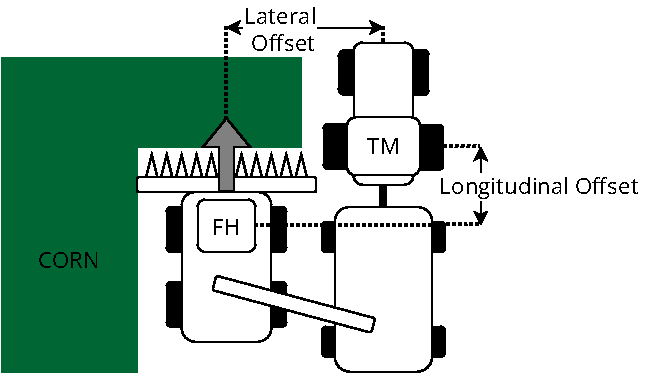
\includegraphics[width=0.95\textwidth]{figures/offset_platoon.pdf}
	\caption{Lateral and longitudinal Offset between the two agricultural machines \ac{FH} and \ac{TM} in a corn harvest scenario}%
	\label{fig:offset}%
\end{figure}

At the same time, the harvesting process is also an example of the video streaming use case. During the harvesting process of the spout of the \ac{FH} must be controlled to set the loading position of the forage into the trailer of the \ac{TM}.

According to \textcite{HMThesis}, different spout guidance and control systems have been developed for this reason, which use a camera attached to the spout to determine via machine vision the fill volume at each point of the trailer and set the spout to fill the empty parts of the trailer accordingly. The author describes the Autofill - system from Claas and the Intellifill - system from CNH Industrial as examples of spout guidance systems. 

Streaming the video of the camera at the spout from the \ac{FH} to the \ac{TM} would be a useful application of the video streaming use case in the harvesting process. If the driver of the \ac{TM} can watch a livestream of the trailer's fill level, he is always informed and knows when the trailer is full so he can drive the feed back to the farm.




Definition Feldhäcksler


Nach Feldhäcksler 1962 ist ein Feldhäcksler eine Lademaschine für fast alle Futterarten:

Heu und

Mais als Grünmais für die tägliche Fütterung und als Silomais
Gras und Klee für die tägliche Fütterung und für die Silage
Heu und Stroh 

Introduction Corn Harvest, Forage Harvesters


\chapter{Analyzing Corn Harvest Process Data}
To gain a better insight into the some requirements for the application ot the \ac{WIC} use cases Platooning and Streaming Services in a corn harvest scenario, I collected GPS tracks of a \ac{FH} and two to three \ac{TM}s harvesting corn on a field in Germany on two days in September. For this, I placed tablets in the driver's cabs of the agricultural vehicles, which recorded the NMEA data stream of the GPS every second. 

The workflow for collecting the corn harvest process data was as follows. 
I handed out the tablets to the drivers, which left the farm with the tablets in the driver's cabs to drive to the field in the morning. The tablets recorded position and speed of the \ac{FH} and the \ac{TM}s all day long. During breaks, the tablets continued to capture NMEA data stream of their GPS even if the positions and speed did not change.

First, I anonymized the timestamps of the recorded NMEA files by deleting the first data points of the log files for the timestamps where the recorded accuracy of all log files was not yet less than 2 m. From the time when the accuracy of all log files was less than 2 m, I replaced the timestamp and the date for all further data points with a continuous index.

After that I anonymized the location data by adding a random offset to the GPS coordinates. Damit wurden die Flächen auf eine zufällige Stelle auf der Welt verschoben.

The goal of analysing the corn harvest data was to investigate the machines move in the working scenarios relative to each other. The speed and distance of the machines in tracked data may result in new use case requirements for e.g. latency or communication range. The machinery movement profile can be used to identify when shadowing effects may occur in the work scenario or when machines meet in the field.
Da im Harvest Process das overloading scenario das work scenario ist, musste ich zunächst einen intelligenten Algorithmus entwickeln. Dieser kann in den aufgezeichneten Daten overloading scenarios entdecken.

Dazu habe ich mir zu Beginn Dashboard mit dem python Framework \textit{Dash}\footnote{https://dash.plotly.com/introduction Accessed: 5.12.2022} gebaut. Darin habe ich mir über auf einer Karte zunächst für jede Maschine alle Positionen in einer Polyline geplotted. Über einen Slider konnte man dann ein Zeitinterval festlegen, für welches welches man den Geschwindigkeits - und Positionsverlauf genauer anschauen möchte. Zusätzlich konnte man auswählen, welche \ac{TM}s man zusätzlich zum \ac{FH} angezeigt haben möchte. Nur die ausgewählten \ac{TM}s und der \ac{FH} wurden dann für das Zeitinterval betrachtet. Die Positionen des ausgewählten Zeitintervals habe ich ebenso in eine Karte als Polyline geplotted. Zusätzlich wurden für das Zeitinterval die Distanz der ausgewählten \ac{TM}s zum \ac{FH}, die Geschwindigkeitsdifferenz zwischen den \ac{TM}s und \ac{FH} und die jeweiligen Geschwindigkeiten der ausgewählten Maschinen in Graphen als Zeitverläufe dargestellt. 

Über diese Visualisierung der Daten konnte ich mir zunächst einen Überblick über das Verhalten der Maschinen vor, während, nach dem Overloading scenario schaffen. Dabei ist im überblick zu erkennen, dass der \ac{FH} nahezu durchgängig neben einer \ac{TM} fährt und mit ihr im Overloading Prozess ist.
Dabei kann der \ac{FH} immer mal auf der Stelle stehen, wenn das Schneidewerk verstopft ist oder ein Übergang ist, wo die volle \ac{TM} sich vom \ac{FH} entfernt und eine leere \ac{TM} zum \ac{FH} aufschließt, um Corn aufzunehmen. 
\begin{figure}%
	\centering
	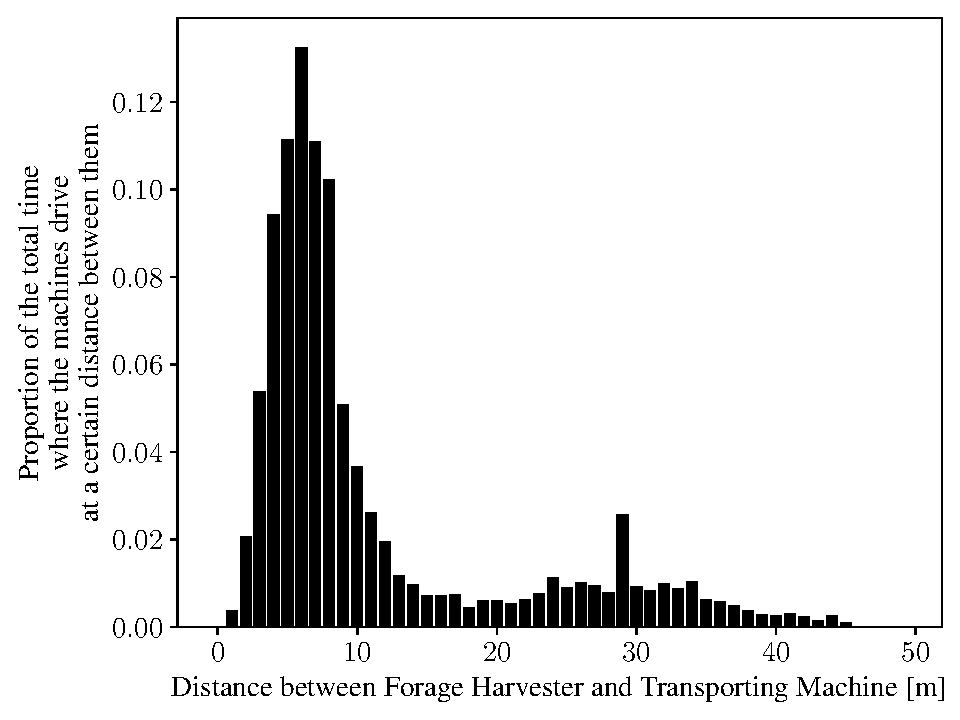
\includegraphics[width=0.85\textwidth]{figures/distanceHarvestSzenario.pdf}
	\caption{Distribution of time proportions where a given distance was between \ac{FH} and \ac{TM} in a harvest platoon scenario.}%
	\label{fig:distance}%
\end{figure}
\begin{figure}%
	\centering
	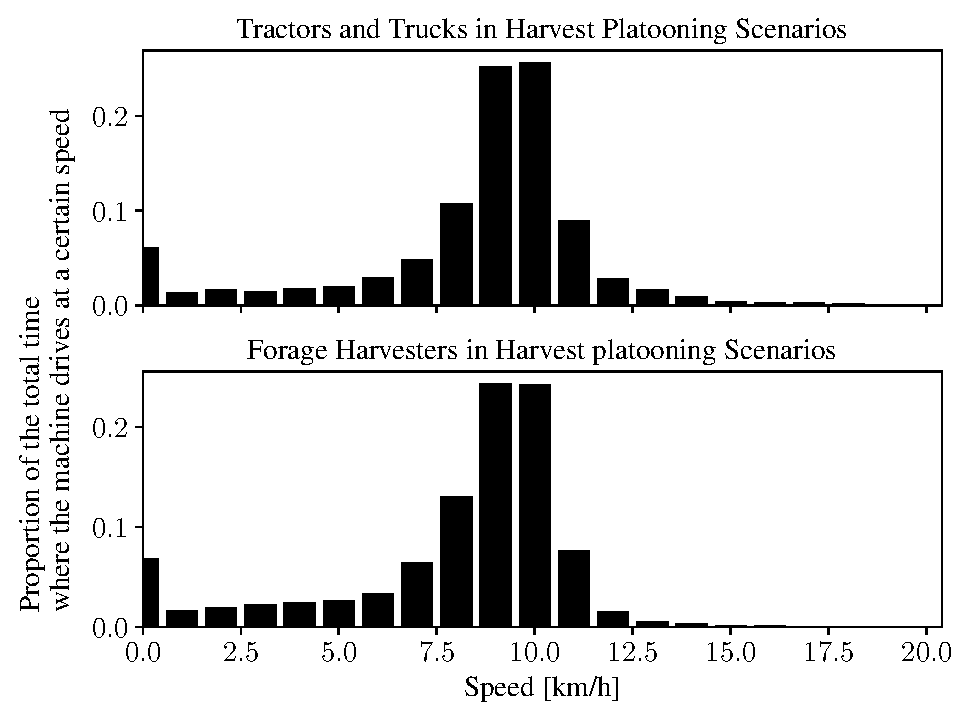
\includegraphics[width=0.85\textwidth]{figures/speedHarvestSzenario.pdf}
	\caption{Distribution of time proportions where FH and TM drove with a certain speed in a harvest platoon scenario}%
	\label{fig:speed}%
\end{figure}

\textcite{klingler_agriculture_2018} hat bereits die Suitability von IEEE 802.11p für \ac{WIC} untersucht. Dabei haben die Autoren festgestellt, dass es im Harvest scenario zu shadowing effecten kommen kann, wo die RSS plötzlich sehr stark singt. Die Autoren erklären sich das, weil entweder ein anderen Traktor oder der Spout des \ac{FH} sich in der \ac{LOS} befunden haben. 

Um einen Überblick zu bekommen, wo sich der \ac{TM} im Overloading Process im Verhältnis zum \ac{FH} befindet, habe ich die aufgezeichneten Positionsdaten aus dem Corn Harvest Scenario untersucht. Dazu habe ich jeden Zeitpunkt in im Overloading Scenario das relative Bearing zwischen dem Heading des \ac{FH} und der \ac{TM} berechnet. Das relative Bearing ist der Winkel zwischen B und dem Heading es Punktes A, wie in \autoref{fig:bearing_plain} zu sehen ist.  

Heading Annahme Vorwärts Fahrt. Ansonsten Überprüfen und nochmal Einzelfahrt plotten und anschauen. 
Wie oft dreht sich das Heading ?
Möglicherweise Rückwärtsfahrt erkennen? 



\begin{figure}%
	\centering
	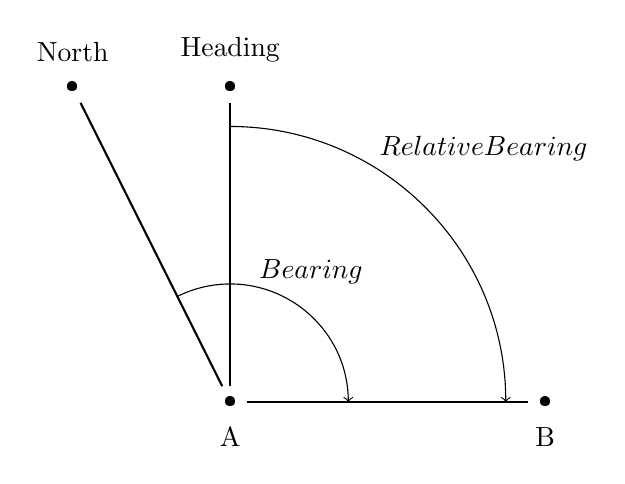
\begin{tikzpicture}
		\node[label=below:A](a) at (0,0) {\textbullet};
		\node[label=above:North](d) at (-2,4) {\textbullet};
		\node[label=above:Heading](c) at (0,4) {\textbullet};
		\node[label=below:B](b) at (4,0) {\textbullet};
		\draw [thick] (a) -- (b);
		\draw [thick] (a) -- (c);
		\draw [thick] (a) -- (d);
		\draw
		pic["$Bearing$", draw, <-,angle eccentricity=1.3, angle radius=1.5cm]
		{angle=b--a--d}
		pic["$Relative Bearing$", draw, <-, angle eccentricity=1.3, angle radius=3.5cm]
		{angle=b--a--c};
	\end{tikzpicture}
	\caption{Relative and True bearing between A and B}%
	\label{fig:bearing_fh_tm}%
\end{figure}

\begin{figure}%
	\centering
	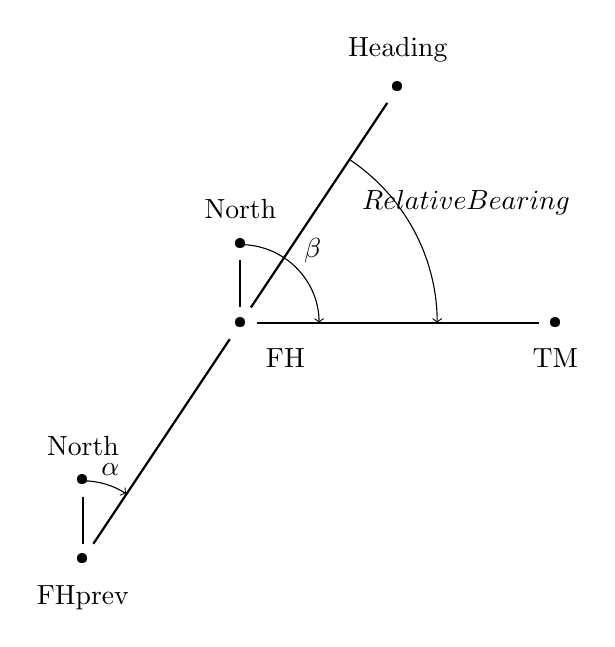
\begin{tikzpicture}
		\node[label=below right:FH](a) at (0,0) {\textbullet};
		\node[label=above:North](d) at (0,1) {\textbullet};
		\node[label=above:Heading](c) at (2,3) {\textbullet};
		\node[label=below:TM](b) at (4,0) {\textbullet};
		\node[label=below:FHprev](e) at (-2,-3) {\textbullet};
		\node[label=above:North](f) at (-2,-2) {\textbullet};
		\draw [thick] (a) -- (b);
		\draw [thick] (a) -- (c);
		\draw [thick] (a) -- (d);
		\draw [thick] (a) -- (e);
		\draw [thick] (e) -- (f);
		\draw 
		pic["$\beta$", draw, <-,angle eccentricity=1.3, angle radius=1.0cm]
		{angle=b--a--d}
		pic["$\alpha$", draw, <-,angle eccentricity=1.2, angle radius=1.0cm]
		{angle=a--e--f}
		pic["$Relative Bearing$", draw, <-, angle eccentricity=1.3, angle radius=2.5cm]
		{angle=b--a--c};
	\end{tikzpicture}
	\caption{Relative bearing between \ac{FH} and \ac{TM} which is calculated using the previous location of \ac{FH} by the difference of $\beta$ minus $\alpha$}%
	\label{fig:bearing_plain}%
\end{figure}





\begin{figure}%
	\centering
	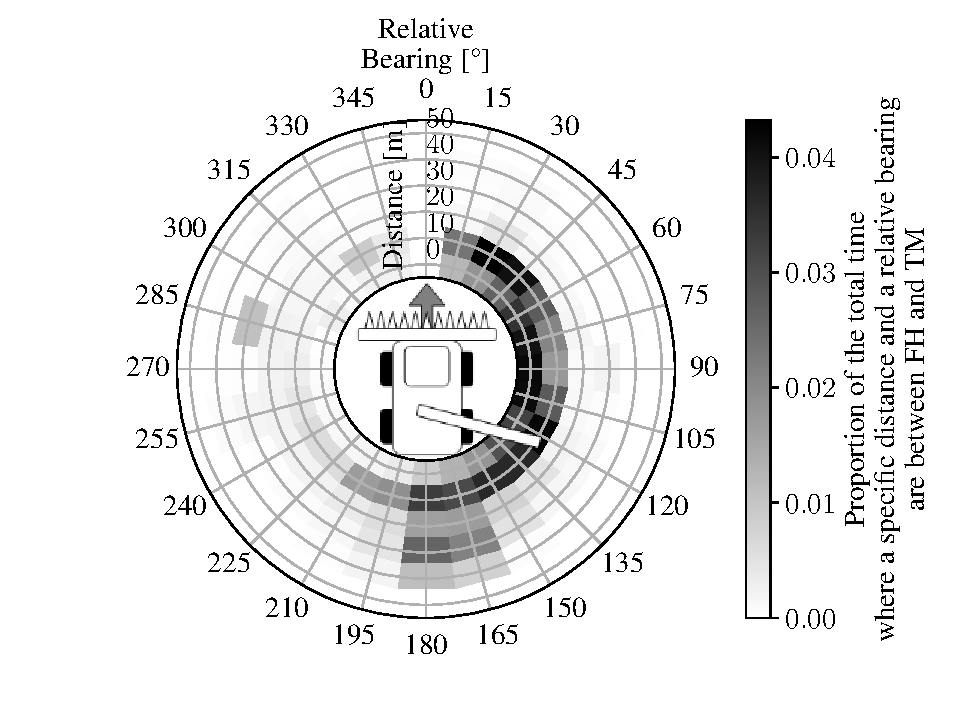
\includegraphics[width=0.99\textwidth]{figures/bearingHarvestScenario.pdf}
	\caption{Distribution of time proportion at specific distances and relative bearings between \ac{FH} and \ac{TM}}%
	\label{fig:bearing}%
\end{figure}
\chapter{Field Measurements}


\chapter{Developed architecture / System design / Implementation / ...}


\begin{itemize}
\item describe everything you yourself did (as opposed to the fundamentals chapter, which explains what you built on)
\item start with a theoretical approach
\item describe the developed system/algorithm/method from a high-level point of view
\item go ahead in presenting your developments in more detail
\item recommended length: approximately one third of the thesis.
\end{itemize}

\chapter{Simulation}

Propagation Model:
 Two Ray Ground only mathematics Rappaport
 Jakes Model
 Three Log Distance
 
 
 Data Simulation
 


\chapter{Evaluation}


\begin{itemize}
\item measurement setup / results / evaluation / discussion
\item whatever you have done, you must comment it, compare it to other systems, evaluate it
\item usually, adequate graphs help to show the benefits of your approach
\item each result/graph must not only be described, but also discussed (What's the reason for this peak? Why have you observed this effect? What does this tell about your architecture/system/implementation?)
\item recommended length: approximately one third of the thesis.
\end{itemize}



\chapter{Conclusion}


\begin{itemize}
\item summarize again what your paper did, but now emphasize more the results, and comparisons
\item write conclusions that can be drawn from the results found and the discussion presented in the paper
\item future work (be very brief, explain what, but not much how, do not speculate about results or impact)
\item recommended length: one page.
\end{itemize}



\cleardoublepage

\listofabbreviations
\clearpage

\listoffigures
\clearpage

\listoftables
\clearpage

\printbibliography

\end{document}
